The dynamic project naming script in the code listing for the \texttt{gh}
code example is shown In Figure \ref{fig:naming-code-gh}.  This is used to create a project with the naming convention:\\\\
\texttt{<first 6 or less chars of organization>\_<repo name>}\\

\begin{figure}[h]
    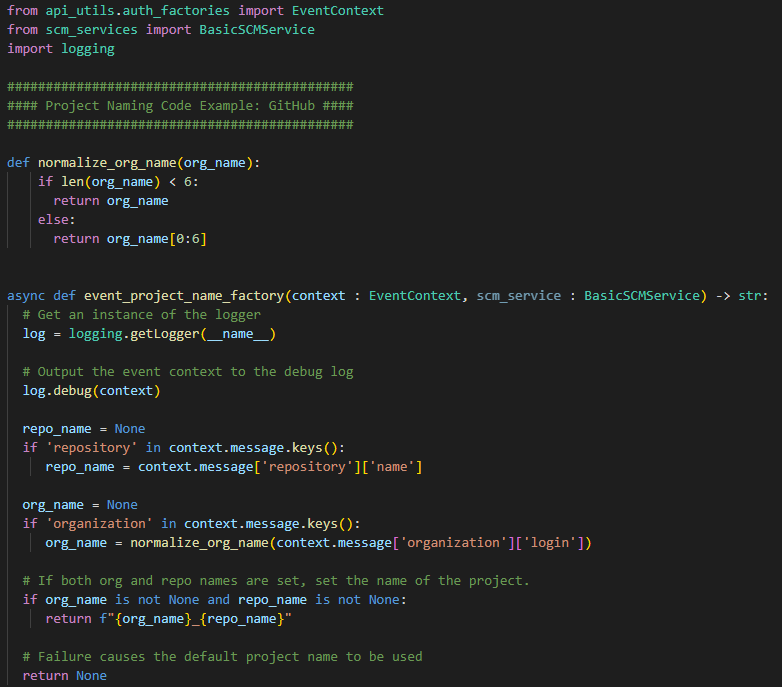
\includegraphics[width=\textwidth]{graphics/naming-code-gh.png}
    \caption{GitHub Custom Project Naming Code Example}
    \label{fig:naming-code-gh}
\end{figure}
